\appendix
%\chapter{Proof of Theorem 1}\label{appendix1}
\chapter{動作再現実験における実験結果}\label{appendix1}

動作の再現実験における、教示誤差と再現誤差の関係を図\ref{figure:errors}に示す。
ここで、横軸は教示誤差の分散、縦軸は再現誤差の標準偏差を表す。
各教示誤差において、教示動作からの学習、再現を行った際の再現誤差を50回ずつ実験を行った。適切な観点が選択されている場合、教示誤差と再現誤差の分散が等しくなることが期待される。即ち各グラフにおいて教示誤差$t$、再現誤差$r$に関して、
\[
	r = \sqrt{t}
\]
という関係が満たされていることが期待される。実際のグラフ中には、無理関数に従うように見える結果と、相関が見られ難い結果が存在している。これらの違いと判別基準については付録\ref{appendix2}で説明する。

%%%%%%%%%%%%%%%%%%%%%%%%%%%%%%%%%%%%%%%%%%%%%%%%%%%%%%%%%%%%%%%%%%%%%%%%%%%%%%%%%%%%%%%%%%%%%%%%%%%%%%%
	\begin{figure}
%中央ぞろえ
		\begin{center}
			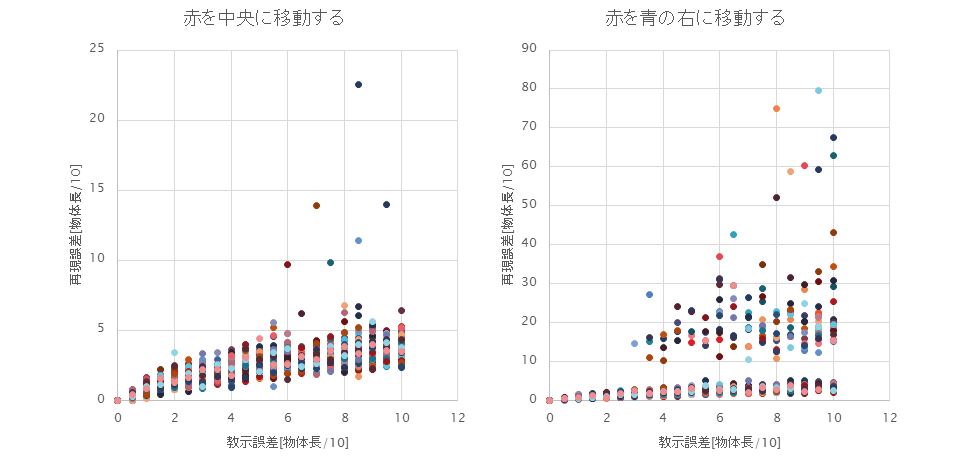
\includegraphics[width=15.5cm]{chart6.png} \\ %eXの基本として, \\ で緊急改行ができる。(今回の場合や行列などを除き、あまり使わない)
			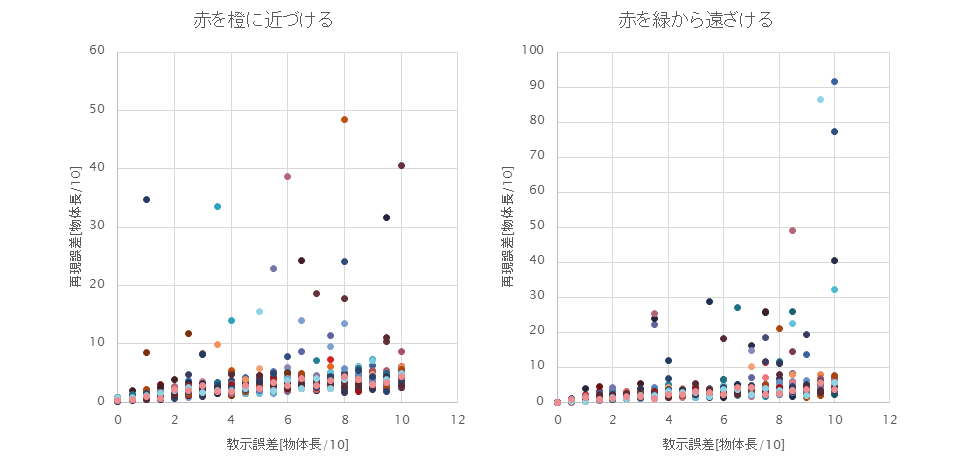
\includegraphics[width=15.5cm]{chart7.png} \\ %eXの基本として, \\ で緊急改行ができる。(今回の場合や行列などを除き、あまり使わない)
			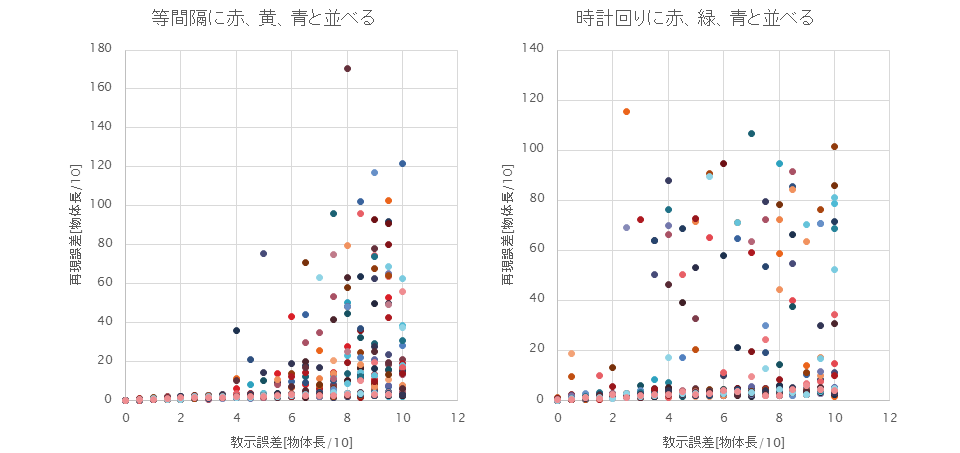
\includegraphics[width=15.5cm]{chart8.png} \\ %eXの基本として, \\ で緊急改行ができる。(今回の場合や行列などを除き、あまり使わない)
			\caption{教示誤差と再現誤差}
			\label{figure:errors}
		\end{center}
	\end{figure}
%%%%%%%%%%%%%%%%%%%%%%%%%%%%%%%%%%%%%%%%%%%%%%%%%%%%%%%%%%%%%%%%%%%%%%%%%%%%%%%%%%%%%%%%%%%%%%%%%%%%%%%



\chapter{動作再現における観点推定の成否の判定}\label{appendix2}

教示動作から学習したモデルを用いた動作再現を行う際、教示動作自体に誤差が含まれている場合、一つ抜き法によるテスト時に使用するデータも教示動作の一つであるために必然的に誤差が生じる。そのため一つ抜き法により計算された再現誤差が教示誤差に依るものなのか誤学習に依るものなのかを区別する基準が必要である。ここでは正規分布から生成された誤差を含む教示動作から適切に学習された場合に再現誤差も正規分布に従うことを示し、正規分布の性質から観点推定の成否の基準値を設定する。
まず、適切な観点(原点となる参照点と座標系)からの$N$回分の各教示動作における目標位置$Θ=\{θ_{1} , θ_{2} , \ldots , θ_{N}\}$に対し、$Θ$を用いた一つ抜き法による評価値を次のように求める。
	\begin{equation}
		\label{CrossVaridation}
		Cr(Θ) = \frac{1}{N} \sum_{n=1}^{N} F(θ_{n} | Θ \backslash θ_{n})
	\end{equation}
ここで\ref{CrossVaridation}式の右辺$F(θ_{n} | Θ \backslash θ_{n})$は、$θ_{n}$を除く$Θ$を用いて学習し再現を行った結果の目標位置と$θ_{n}$の誤差を表す。動作再現は選択された観点に割り当てられた正規分布の平均を出力するので、
	\begin{equation}
		\label{F}
		F(θ_{n} | Θ \backslash θ_{n}) = |θ_{n} - mean(Θ \backslash θ_{n})| = |\frac{N}{N-1}(θ_{n} - mean(Θ))|
	\end{equation}
である。ただし$mean(A)$はAの平均とする。\ref{F}式を\ref{CrossVaridation}に代入すると
	\begin{equation}
		\label{Cr2}
		Cr(Θ) = \frac{1}{N} \sum_{n=1}^{N}  |\frac{N}{N-1}(θ_{n} - mean(Θ))|
		 = \frac{N}{N-1}\frac{1}{N}  \sum_{n=1}^{N}  |(θ_{n} - mean(Θ))| 
	\end{equation}
と整理できる。ここで\ref{Cr2}式の右辺$|(θ_{n} - mean(Θ))|$は$θ_{n}$の持つガウス誤差と等しいので、
	\begin{equation}
		\label{Cr3}
		mean(Cr(Θ)) = \frac{N}{N-1} * mean(\frac{1}{N}  \sum_{n=1}^{N}  |(θ_{n} - mean(Θ))| )
		 = \frac{N}{N-1} * mean(|G_{error}|)
	\end{equation}
となる。$2\int_{0}^{\infty}G_{error}(v)dv = \sqrt{\frac{2}{\pi}}σ$であることから、$Cr(Θ)$の平均は
	\begin{equation}
		\label{Cr4}
		mean(Cr(Θ)) = \frac{N}{N-1}\sqrt{\frac{2}{\pi}}σ
	\end{equation}
と求められる。ただし$σ$はガウス誤差の分散である。同様に、
	\begin{equation}
		\label{Cr^2_1}
		mean(Cr(Θ)^2) = \left(\frac{N}{N-1}\right)^2 * mean(|G_{error}|^2) 
		= 2\int_{0}^{\infty}\frac{x^2}{\sqrt{2\pi}σ}e^{-\frac{x^2}{2σ^2}}dx
	\end{equation}
であり、これを計算することで、
	\begin{equation}
		\label{Cr^2_2}
		mean(Cr(Θ)^2) = \left(\frac{N}{N-1}\right)^2 σ^2
	\end{equation}
が得られる。\ref{Cr4}式と\ref{Cr^2_2}式から、$Cr(Θ)$の標準偏差は、
	\begin{equation}
		\sqrt{V(Cr(Θ))} = \sqrt{mean(Cr(Θ)^2) - \left(mean(Cr(Θ))\right)^2} = \frac{N}{N-1}\sqrt{\frac{\pi-2}{\pi}}σ
	\end{equation}
と求められる。平均$m$、分散$σ$の正規分布に従うデータ$θ$に対して$|θ-m|>3σ$となる確率は99.73\%となることが知られている。このような$θ$は、適切な観点でない異なる分布から生起されたとし、観点の推定自体を誤っていると考えることで、観点推定の成否を判定し評価することができる。今回の実験において$θ>0$であるため、基準値$θ_{border}$を、
	\begin{equation}
		θ_{border} = mean(Cr(Θ))+3\sqrt{V(Cr(Θ))}≒2.8959σ
	\end{equation}
と定め、これ以上の再現誤差が生じた結果について観点推定失敗と定めた。



%\chapter{Proof of Theorem 2}\label{appendix2}
%\chapter{定理2の証明}\label{appendix2}
